\newpage
\section{Аналитические отчеты}

Для получения в \tmisp~отчетов по введенной информации нужно на панели навигации в левой части страницы щелкнуть по пиктограмме \dm{Аналитические отчеты}. В основной части страницы отобразится список отчетов, доступных пользователю (Рисунок \ref{img_rep_main}). В зависимости от роли и полномочий пользователя в системе, список отчетов может отличаться.

\begin{figure}[ht]\centering
	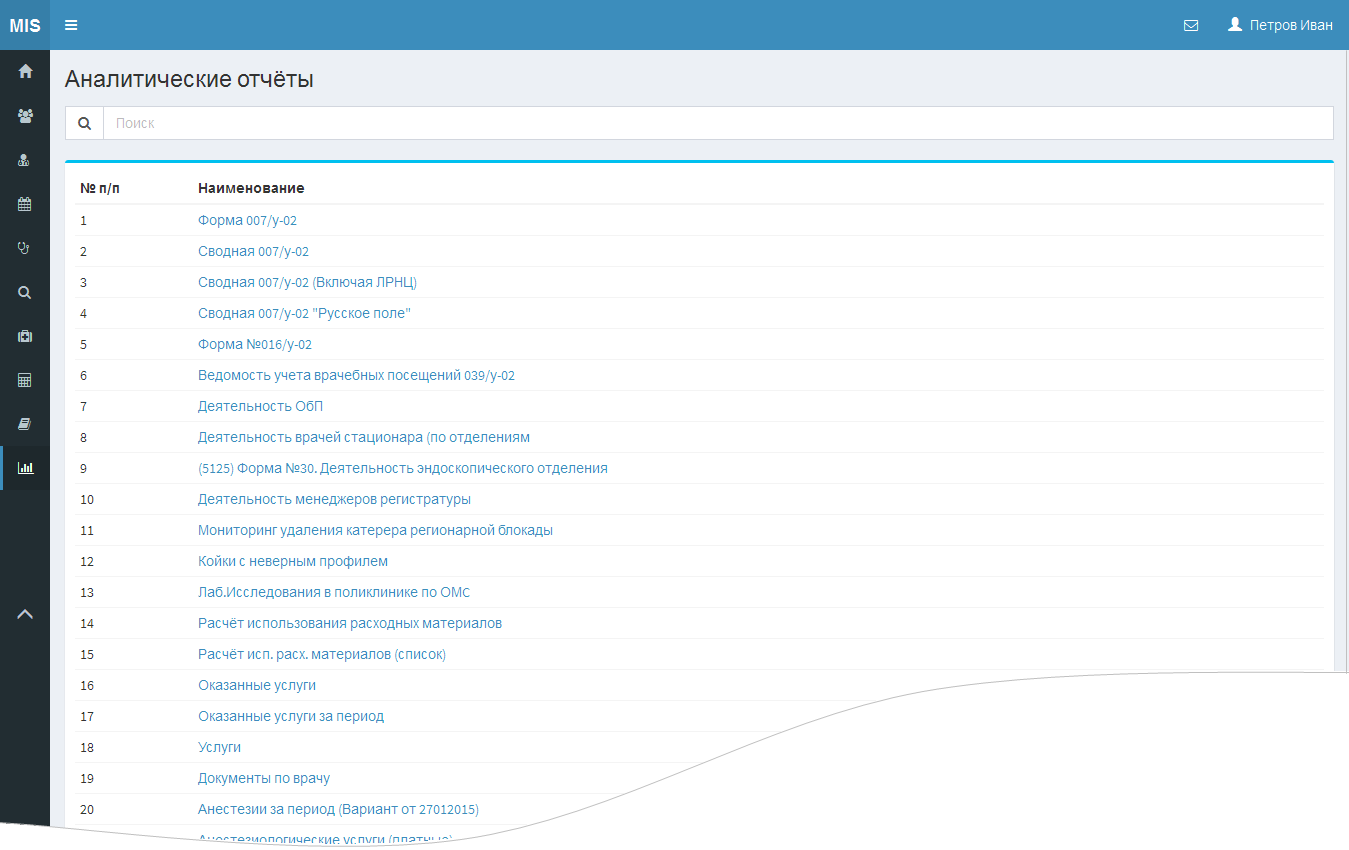
\includegraphics[width = 1\textwidth ,keepaspectratio]{rep_main}
	\caption{Страница <<Аналитические отчеты>>}
	\label{img_rep_main}
\end{figure}

Если список отчетов слишком большой, для его просмотра можно воспользоваться полосой прокрутки, расположенной по правому краю страницы, либо колесом прокрутки мыши.

Для запуска формирования отчета следует щелкнуть левой кнопкой мыши по его нименованию в списке и в открывшемся всплывающем окне (Рисунок \ref{img_rep_dialog}) задать параметры отчета. Параметры могут быть различных типов: параметры типа <<дата>> выбираются из календаря, некоторые параметры могут выбираться из раскрывающегося списка или вводиться вручную с клавиатуры. При выборе параметра из справочника, в поле предусмотрен поиск (см. раздел \ref{gen_filtr}). После того как все параметры указаны, становится доступной кнопка \btn{Печать}. После нажатия на данную кнопку, на экране появляется форма предварительного просмотра отчета (Рисунок \ref{img_rep_rep39}), который можно направить на принтер.

\begin{figure}[ht]\centering
	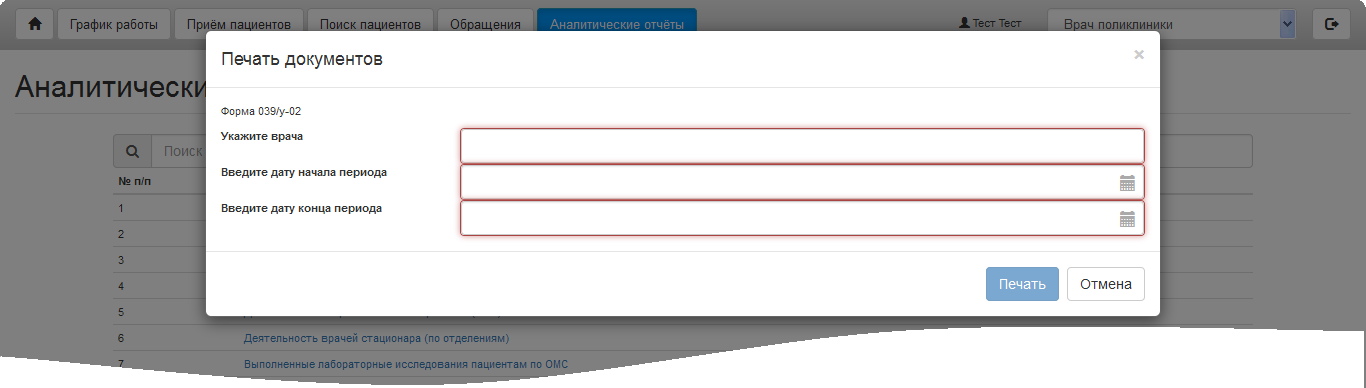
\includegraphics[width = 1\textwidth ,keepaspectratio]{rep_dialog}
	\caption{Параметры аналитического отчета}
	\label{img_rep_dialog}
\end{figure}

\begin{figure}[!ht]\centering
	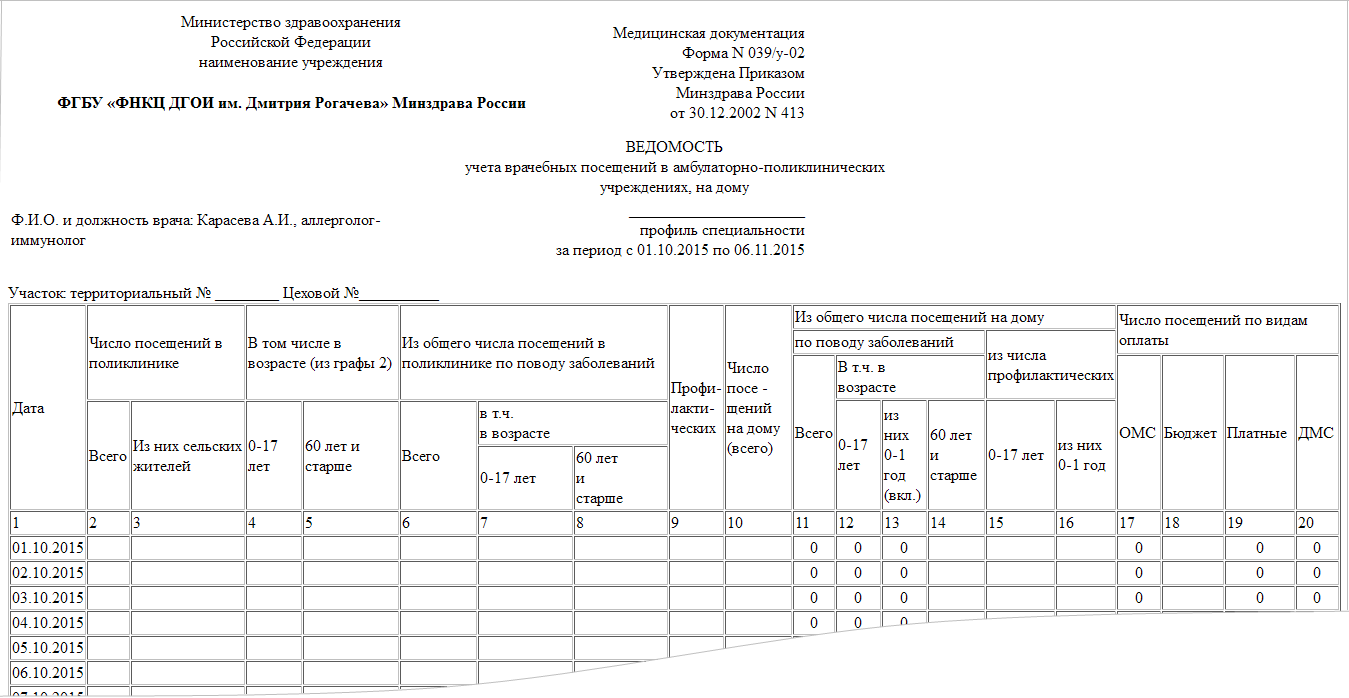
\includegraphics[width = 1\textwidth ,keepaspectratio]{rep_rep39}
	\caption{Страница предварительного просмотра отчета <<Форма 039/2. Ведомость учета врачебных посещений в амбулаторно-поликлинических учреждениях, на дому>>}
	\label{img_rep_rep39}
\end{figure}